\documentclass[11pt,letterpaper]{article}

% ============================================================================
% PACKAGES
% ============================================================================
\usepackage[utf8]{inputenc}
\usepackage[T1]{fontenc}
\usepackage{helvet}
\renewcommand{\familydefault}{\sfdefault}
\usepackage[margin=0.5in, top=0.5in, bottom=0.4in]{geometry}
\usepackage{xcolor}
\usepackage{tikz}
\usepackage{tcolorbox}
\usepackage{multicol}
\usepackage{enumitem}
\usepackage{parskip}
\usepackage{hyperref}

\usetikzlibrary{shapes.geometric, arrows.meta, positioning, calc, backgrounds, fit, decorations.pathreplacing}

% ============================================================================
% COLOR DEFINITIONS
% ============================================================================
\definecolor{humangate}{HTML}{27AE60}       % Green - Human gates
\definecolor{agentwork}{HTML}{3498DB}       % Blue - Agent work
\definecolor{reviewloop}{HTML}{9B59B6}      % Purple - Review/feedback
\definecolor{kanban}{HTML}{E67E22}          % Orange - Kanban states
\definecolor{darktext}{HTML}{2C3E50}        % Dark text
\definecolor{lightbg}{HTML}{F5F6F7}         % Light background
\definecolor{claude}{HTML}{CC785C}          % Claude orange-brown
\definecolor{gemini}{HTML}{4285F4}          % Gemini blue
\definecolor{codex}{HTML}{10A37F}           % OpenAI green

% ============================================================================
% DOCUMENT
% ============================================================================
\pagestyle{empty}
\setlength{\parskip}{0.3em}
\setlist{nosep, leftmargin=1.2em, itemsep=0.2em}

\begin{document}

% Header
\noindent
\begin{minipage}[t]{0.7\textwidth}
\textcolor{darktext}{\LARGE\textbf{AI-Assisted Development Workflow}}\\[0.2em]
\textcolor{darktext!70}{Human oversight with composable agent actions}
\end{minipage}%
\hfill
\begin{minipage}[t]{0.25\textwidth}
\raggedleft
\textcolor{darktext!50}{\small Agent Kanban Workflow}
\end{minipage}

\vspace{0.4em}
\hrule height 0.5pt
\vspace{0.5em}

% Main workflow diagram
\begin{center}
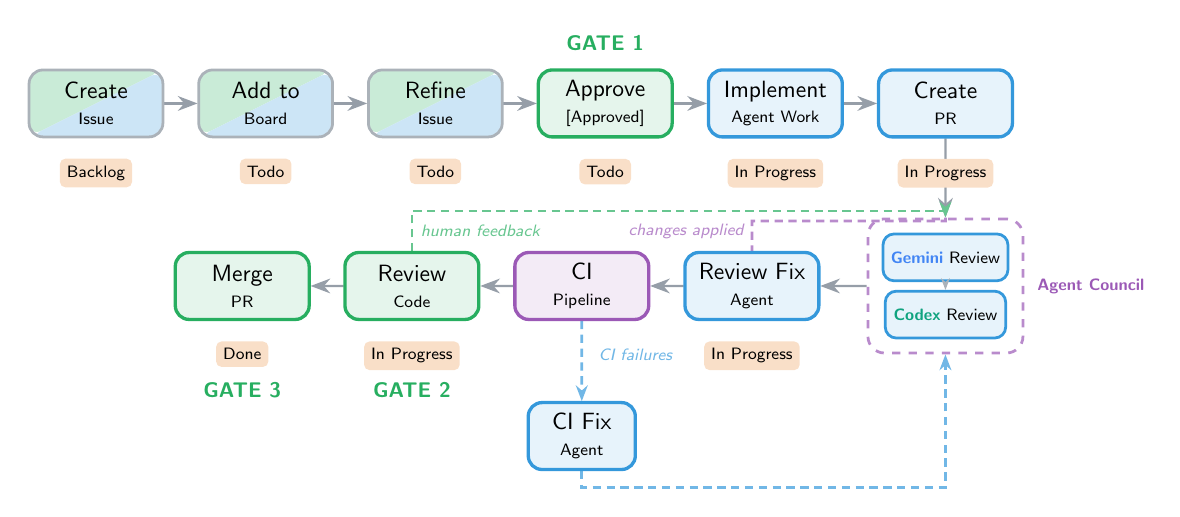
\begin{tikzpicture}[scale=0.85, transform shape,
  node distance=0.7cm and 0.5cm,
  every node/.style={font=\sffamily},
  stage/.style={rectangle, rounded corners=5pt, minimum height=1cm, minimum width=2cm, align=center, line width=1.2pt},
  human/.style={stage, draw=humangate, fill=humangate!12},
  agent/.style={stage, draw=agentwork, fill=agentwork!12},
  review/.style={stage, draw=reviewloop, fill=reviewloop!12},
  smallagent/.style={rectangle, rounded corners=4pt, draw=agentwork, fill=agentwork!12, minimum height=0.7cm, minimum width=1.8cm, align=center, line width=1pt},
  kanban/.style={rectangle, rounded corners=2pt, fill=kanban!25, font=\scriptsize\sffamily, inner sep=3pt},
  arrow/.style={-{Stealth[length=2.5mm]}, thick, color=darktext!50},
  looparrow/.style={-{Stealth[length=2mm]}, line width=1pt, color=reviewloop!80, densely dashed}
]

% === ROW 1: Forward Path (Left to Right) ===
% Hybrid style: diagonal split - green (human) top-left, blue (agent) bottom-right
\node[stage, draw=darktext!40, line width=1pt,
      path picture={
        \fill[humangate!25] (path picture bounding box.north west) --
              (path picture bounding box.north east) --
              (path picture bounding box.south west) -- cycle;
        \fill[agentwork!25] (path picture bounding box.south east) --
              (path picture bounding box.north east) --
              (path picture bounding box.south west) -- cycle;
      }] (issue) {Create\\[-0.1em]{\scriptsize Issue}};

% Mixed human+agent node for board (diagonal split)
\node[stage, right=of issue, draw=darktext!40, line width=1pt,
      path picture={
        \fill[humangate!25] (path picture bounding box.north west) --
              (path picture bounding box.north east) --
              (path picture bounding box.south west) -- cycle;
        \fill[agentwork!25] (path picture bounding box.south east) --
              (path picture bounding box.north east) --
              (path picture bounding box.south west) -- cycle;
      }] (triage) {Add to\\[-0.1em]{\scriptsize Board}};

\node[stage, right=of triage, draw=darktext!40, line width=1pt,
      path picture={
        \fill[humangate!25] (path picture bounding box.north west) --
              (path picture bounding box.north east) --
              (path picture bounding box.south west) -- cycle;
        \fill[agentwork!25] (path picture bounding box.south east) --
              (path picture bounding box.north east) --
              (path picture bounding box.south west) -- cycle;
      }] (refine) {Refine\\[-0.1em]{\scriptsize Issue}};
\node[human, right=of refine] (approve) {Approve\\[-0.1em]{\scriptsize [Approved]}};
\node[agent, right=of approve] (implement) {Implement\\[-0.1em]{\scriptsize Agent Work}};
\node[agent, right=of implement] (createpr) {Create\\[-0.1em]{\scriptsize PR}};

% Arrows (on background so kanban labels appear on top)
\begin{scope}[on background layer]
\draw[arrow] (issue) -- (triage);
\draw[arrow] (triage) -- (refine);
\draw[arrow] (refine) -- (approve);
\draw[arrow] (approve) -- (implement);
\draw[arrow] (implement) -- (createpr);
\end{scope}

% Gate label
\node[above=0.15cm of approve, font=\small\bfseries\color{humangate}] {GATE 1};

% Kanban below row 1
\node[kanban, below=0.3cm of issue] {Backlog};
\node[kanban, below=0.3cm of triage] {Todo};
\node[kanban, below=0.3cm of refine] {Todo};
\node[kanban, below=0.3cm of approve] {Todo};
\node[kanban, below=0.3cm of implement] {In Progress};
\node[kanban, below=0.3cm of createpr] {In Progress};

% === ROW 2: Review Path (Right to Left) ===

% Agent Council -- composable actions in dashed group
\node[smallagent] (gemini-act) at ($(createpr) + (0, -2.3)$)
  {\scriptsize\textcolor{gemini}{\textbf{Gemini}} Review};
\node[smallagent, below=0.12cm of gemini-act] (codex-act)
  {\scriptsize\textcolor{codex}{\textbf{Codex}} Review};

% Dashed group around council actions
\node[draw=reviewloop!70, dashed, rounded corners=6pt, line width=1pt,
      inner sep=5pt, fit=(gemini-act)(codex-act),
      label={[font=\scriptsize\sffamily\bfseries, text=reviewloop, anchor=west, xshift=2pt]right:Agent Council}] (council) {};

% Arrow within council (Gemini feeds Codex)
\draw[-{Stealth[length=1.5mm]}, thin, color=darktext!40] (gemini-act) -- (codex-act);

% Other row 2 nodes aligned to council center
% Shift all row 2 nodes slightly left to give breathing room from council
\node[agent] at ($(implement |- council.center) + (-0.35, 0)$) (autofix) {Review Fix\\[-0.1em]{\scriptsize Agent}};
\node[review] at ($(approve |- council.center) + (-0.35, 0)$) (ci) {CI\\[-0.1em]{\scriptsize Pipeline}};
\node[human] at ($(refine |- council.center) + (-0.35, 0)$) (humanrev) {Review\\[-0.1em]{\scriptsize Code}};
\node[human] at ($(triage |- council.center) + (-0.35, 0)$) (merge) {Merge\\[-0.1em]{\scriptsize PR}};

% CI Failure Auto-Fix box (below CI Pipeline)
\node[agent, below=1.2cm of ci, minimum width=1.6cm] (cifix) {CI Fix\\[-0.1em]{\scriptsize Agent}};

% Main flow arrows (on background so kanban labels appear on top)
\begin{scope}[on background layer]
\draw[arrow] (createpr) -- (council);
\draw[arrow] (council) -- (autofix);
\draw[arrow] (autofix) -- (ci);
\draw[arrow] (ci) -- (humanrev);
\draw[arrow] (humanrev) -- (merge);
\end{scope}

% Kanban below row 2
\node[kanban, below=0.3cm of autofix] {In Progress};
\node[kanban, below=0.3cm of humanrev] {In Progress};
\node[kanban, below=0.3cm of merge] {Done};

% Gate labels row 2
\node[below=0.8cm of humanrev, font=\small\bfseries\color{humangate}] {GATE 2};
\node[below=0.8cm of merge, font=\small\bfseries\color{humangate}] {GATE 3};

% === FEEDBACK LOOPS ===
\begin{scope}[on background layer]
% Review Fix -> back to Agent Council (changes applied restart pipeline)
% Path: up from autofix, horizontal right to above council, down into council
\coordinate (fix-rise) at ($(autofix.north) + (0, 0.45)$);
\coordinate (council-drop) at (council.north |- fix-rise);
\draw[-, line width=1pt, color=reviewloop!70, densely dashed]
  (council.north) -- (council-drop) -- (fix-rise) -- (autofix.north);
% Label on the horizontal segment, below the line (next to "human feedback")
\node[font=\scriptsize\color{reviewloop!70}\itshape, anchor=east] at ($(autofix.north) + (0, 0.3)$) {changes applied};

% Human review can request changes -> back to council
\draw[looparrow, humangate!70] (humanrev.north) -- ++(0,0.6)
  node[pos=0.5, right, font=\scriptsize\color{humangate!70}\itshape] {human feedback}
  -| (council.north);

% CI failure loop (down to CI Fix, then below back to council)
\draw[looparrow, agentwork!70] (ci.south) -- (cifix.north);
\draw[looparrow, agentwork!70] (cifix.south) -- ++(0,-0.25) -| (council.south);
\end{scope}

% CI failure label
\node[below=0.3cm of ci.south, anchor=north, xshift=0.8cm, font=\scriptsize\color{agentwork!70}\itshape] {CI failures};

\end{tikzpicture}
\end{center}

\vspace{0.1em}

% Legend bar
\begin{center}
\fcolorbox{lightbg}{lightbg}{%
\begin{tabular}{@{}c@{\hspace{0.8em}}c@{\hspace{0.8em}}c@{\hspace{0.8em}}c@{\hspace{0.8em}}c@{}}
\tikz\fill[humangate!35, rounded corners=2pt] (0,0) rectangle (0.4,0.25); \textsf{\small Human} &
\tikz\fill[agentwork!35, rounded corners=2pt] (0,0) rectangle (0.4,0.25); \textsf{\small Agent} &
\tikz{\fill[humangate!25] (0,0.25) -- (0.4,0.25) -- (0,0) -- cycle; \fill[agentwork!25] (0.4,0) -- (0.4,0.25) -- (0,0) -- cycle;} \textsf{\small Hybrid} &
\tikz\fill[reviewloop!35, rounded corners=2pt] (0,0) rectangle (0.4,0.25); \textsf{\small Automation} &
\tikz\fill[kanban!40, rounded corners=2pt] (0,0) rectangle (0.4,0.25); \textsf{\small Kanban}
\end{tabular}%
}
\end{center}

\vspace{0.2em}

% Three-column content
\begin{multicols}{3}
\raggedright

% Column 1: Human Gates
\textcolor{humangate}{\Large\textbf{Human Gates}}
\vspace{0.3em}

\textbf{Three checkpoints} for oversight:

\begin{enumerate}[label=\textbf{\arabic*.}, leftmargin=1.5em, itemsep=0.3em]
  \item \textbf{Approve Work}\\
        {\small \texttt{[Approved]} triggers agent}
  \item \textbf{Code Review}\\
        {\small Can request changes $\rightarrow$ loops back}
  \item \textbf{Merge PR}\\
        {\small Final merge decision}
\end{enumerate}

\vspace{0.3em}

{\small Both humans and agents can create issues. \texttt{.agents.yaml} defines who can approve and review.}

\vspace{0.4em}
\textcolor{reviewloop}{\Large\textbf{Composable Actions}}
\vspace{0.3em}

Each review stage is a reusable GitHub Action:

\begin{itemize}[leftmargin=1.2em, itemsep=0.3em]
  \item \textcolor{gemini}{\textbf{gemini-review}} -- Security \& architecture
  \item \textcolor{codex}{\textbf{codex-review}} -- Code patterns \& quality
  \item \textcolor{claude}{\textbf{pr-review-fix}} -- Auto-fix from reviews
\end{itemize}

\vspace{0.3em}
{\small Actions compose via artifacts. Each uploads its review; downstream actions consume them. Mix and match for different pipelines.}

\columnbreak

% Column 2: Feedback Loops
\textcolor{agentwork}{\Large\textbf{Feedback Loops}}
\vspace{0.3em}

Three automated loops minimize human round-trips:

\vspace{0.3em}
\begin{tcolorbox}[colback=agentwork!10, colframe=agentwork!60, boxrule=0.8pt, arc=3pt, left=6pt, right=6pt, top=4pt, bottom=4pt, title={\small\textbf{Loop 1: Review Cycle}}, fonttitle=\sffamily\bfseries, coltitle=white, colbacktitle=agentwork!70]
{\footnotesize
Council posts reviews\\[0.15em]
$\rightarrow$ Fix agent resolves issues\\[0.15em]
$\rightarrow$ Push restarts council\\[0.15em]
$\rightarrow$ Repeats until clean}
\end{tcolorbox}

\vspace{0.3em}

\begin{tcolorbox}[colback=reviewloop!10, colframe=reviewloop!60, boxrule=0.8pt, arc=3pt, left=6pt, right=6pt, top=4pt, bottom=4pt, title={\small\textbf{Loop 2: CI Failures}}, fonttitle=\sffamily\bfseries, coltitle=white, colbacktitle=reviewloop!70]
{\footnotesize
Format or lint check fails\\[0.15em]
$\rightarrow$ Agent auto-fixes issues\\[0.15em]
$\rightarrow$ Push triggers re-run}
\end{tcolorbox}

\vspace{0.3em}

\begin{tcolorbox}[colback=humangate!10, colframe=humangate!60, boxrule=0.8pt, arc=3pt, left=6pt, right=6pt, top=4pt, bottom=4pt, title={\small\textbf{Loop 3: Human Review}}, fonttitle=\sffamily\bfseries, coltitle=white, colbacktitle=humangate!70]
{\footnotesize
Human requests changes\\[0.15em]
$\rightarrow$ Back to council review}
\end{tcolorbox}

\vspace{0.3em}
\textbf{Safety mechanisms:}
\begin{itemize}[leftmargin=1.2em, itemsep=0.15em]
  \item {\small Max 5 iterations per agent type}
  \item {\small Only \texttt{agent\_admins} can trigger agents}
\end{itemize}

\columnbreak

% Column 3: Kanban + Key Insight
\textcolor{kanban}{\Large\textbf{Kanban Flow}}
\vspace{0.3em}

Board status tracks workflow progress:

\vspace{0.5em}
\begin{center}
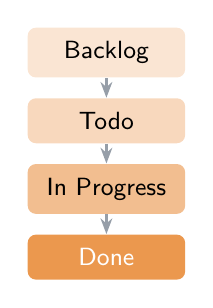
\begin{tikzpicture}[node distance=0.25cm, every node/.style={font=\small\sffamily}]
  \node[fill=kanban!20, rounded corners=3pt, inner sep=5pt, minimum width=2cm] (b) {Backlog};
  \node[fill=kanban!30, rounded corners=3pt, inner sep=5pt, minimum width=2cm, below=of b] (t) {Todo};
  \node[fill=kanban!50, rounded corners=3pt, inner sep=5pt, minimum width=2cm, below=of t] (p) {In Progress};
  \node[fill=kanban!80, rounded corners=3pt, inner sep=5pt, minimum width=2cm, below=of p, text=white] (d) {Done};
  \draw[-{Stealth[length=2mm]}, darktext!50, thick] (b) -- (t);
  \draw[-{Stealth[length=2mm]}, darktext!50, thick] (t) -- (p);
  \draw[-{Stealth[length=2mm]}, darktext!50, thick] (p) -- (d);
\end{tikzpicture}
\end{center}

\vspace{0.4em}
{\small Issues move through stages automatically as agents work. \textbf{Blocked} state available for dependency management.}

\vspace{0.5em}

\begin{tcolorbox}[colback=darktext!8, colframe=darktext!40, boxrule=0.8pt, arc=3pt, left=6pt, right=6pt, top=6pt, bottom=6pt]
\textbf{\large Key Insight}\\[0.3em]
\textcolor{humangate}{\textbf{Humans}} decide \textbf{what} to work on and \textbf{when} to merge.\\[0.3em]
\textcolor{agentwork}{\textbf{Agents}} handle \textbf{how} with composable review actions.
\end{tcolorbox}

\end{multicols}

\vspace{0.2em}
\begin{tcolorbox}[colback=agentwork!5, colframe=agentwork!30, boxrule=0.6pt, arc=3pt, left=8pt, right=8pt, top=4pt, bottom=4pt]
{\small\textbf{Deployment flexibility:} Agent actions can run \textbf{directly on the runner} (as shown here) or dispatch to \textbf{external services} (e.g., AgentCore) by passing the task payload---code diffs, billing reports, quality metrics, or any fetched data from external systems. Organizations can wrap agent endpoints with scaffolding for \textbf{prompt injection protection}, \textbf{cost controls}, and \textbf{usage governance}. The composable action interface stays the same either way.}
\end{tcolorbox}

\end{document}
